\documentclass[a4paper, 11pt]{article} %uiteindelijk 12 doen?

% Language setting
% Replace `english' with e.g. `spanish' to change the document language
\usepackage[english]{babel}

% Set page size and margins
\usepackage[margin=2.2cm]{geometry}
\usepackage{lscape}
% Useful packages
\usepackage{amsmath}
\usepackage{relsize}
\usepackage{mathtools}
\usepackage{diagbox}
\usepackage[table]{xcolor}
\usepackage{xcolor}
\usepackage{graphicx}
\usepackage{setspace}
\usepackage[hidelinks]{hyperref}
\usepackage[textwidth=8em,textsize=small]{todonotes}
\usepackage{multirow} %for tables
\usepackage{multicol} %for tables
\usepackage{subcaption}

\providecommand{\keywords}[1]
{
  \small	
  \textbf{\textit{Keywords---}} #1
}

\renewcommand\topskip{0.1} %space between table header and table


\usepackage[]{apacite}
%\usepackage{natbib} %new addition

\bibliographystyle{apacite}
\doublespacing

\title{Comparing MILC and tree-MILC for estimating and correcting for multiple sources of errors in combined datasets}
\author{Dani\"elle Remmerswaal$^1$ \\\footnotesize{$^1$ Department of Methodology and Statistics, Utrecht University}}


\thispagestyle{empty}

\begin{large}
\noindent Research Master's programme 
Methodology and Statistics for the \newline 
Behavioural, Biomedical and Social Sciences \newline
Utrecht University, the Netherlands \newline
\newline
\newline
\newline
\newline
MSc Thesis Dani\"elle Remmerswaal (4435958) 
\newline
TITLE: "Comparing the performance of MILC and tree-MILC to estimate and correct for multiple sources of errors in combined datasets: A simulation study" 
\newline
May 2022 
\newline
\newline
\newline
\newline
\newline
Supervisors:\newline
Prof. Dr. Ton de Waal \newline
Dr. Laura Boeschoten
\newline
\newline
Second grader: \newline
Prof. Dr. Daniel Oberski
\newline
\newline
\newline
\newline
Preferred journal of publication: Journal of Official Statistics
\newline
Word count: 8199
\newline
\end{large}
\addtocounter{page}{-1}
\clearpage
\pagebreak

\begin{document}
  \maketitle
\begin{abstract} \noindent
National Statistical Offices (NSIs) use surveys and administrative registers to produce statistics. Both datasources are not error-free. Numerous methods exist to correct statistics for errors in single-source data. Linking variables from multiple sources, which is possible on the unit-level by NSIs, together in a combined dataset creates many opportunities such as the application of latent variable modelling (LVM). The Multiple Imputation of Latent classes (MILC) method is a specific use of LVM in combination with multiple imputation to correct errors and produce consistent estimates. It has not been investigated whether MILC is proficient in correcting for multiple sources of errors simultaneously. For this purpose, an adaptation of MILC, tree-MILC is designed. In tree-MILC, the latent class (LC) and imputation step are applied twice with different number of LCs. The performance of MILC and tree-MILC are compared in a simulation study, where the level of selection and measurement errors are varied. Overall, tree-MILC outperforms MILC at estimating statistics for combined datasets in terms of accuracy measures and confidence interval measures. The differences in performance are bigger for datasets with higher levels of errors.

\end{abstract}
\keywords{official statistics, measurement error, MILC, latent class modelling, total survey error}

\section{Introduction}
National Statistical Institutes (NSIs) provide data and produce official statistics on many different social and economic aspects of society. To this end, NSIs traditionally used censuses and surveys. Recently, increasingly more administrative sources are being used as to reduce costs and the response burden \cite{UNECE2011}. While surveys are known to contain errors, registers are often falsely assumed to be error-free. Registers are generally not created for statistical purposes by statistical agencies, but by external owners for administrative purposes \shortcite{Reid_TSE_2017, UNECE2011}. This makes them prone to errors due to mistakes when entering the data, delays in adding changes, and misaligning concepts. For more information, see among others the work of \shortciteA{Groen2012, mixedsourceerrors2016, inconsistentdatasources2017}. Since performing censuses for every statistic is unattainable, and using either registers or surveys as the golden standard is also not flawless, a different approach should be taken to validate data sources to produce consistent statistics. 

Since errors in data sources and data processing can lead to biased and inconsistent statistical estimates, it is important to estimate and correct for errors to produce statistics of high quality. While numerous error-correcting methods exist for single data sources, of which some will be addressed in section \ref{background}, it is also possible to use multiple data sources to correct statistics for errors. A relatively new approach is latent variable modelling (LVM). Here, variables on the same concept are used as indicators in a latent variable model. To estimate for errors in categorical variables, latent class (LC) modelling can be used. In the Multiple Imputation of Latent Classes (MILC) method, LC modelling and multiple imputation (MI) are combined to produce consistent estimates.

The MILC method is developed to estimate and correct for measurement error. In practice when producing statistics, there are often multiple types of errors present in one situation. Inspired by a problem encountered during the production of energy statistics that will be described later, we are interested in situations where selection and measurement errors (see figure \ref{fig:zhang}) occur simultaneously. A question is whether MILC works in these situations, or that a different method is more appropriate. Since we expected MILC to have difficulties, especially for datasets with higher levels of errors, we designed an adaptation of MILC that might be more suitable for situations with multiple sources of errors, and named it tree-MILC. Tree-MILC is inspired by latent class tree (LCT) analysis as developed by \citeA{bergh2018latent} and uses the concept of applying LC models sequentially on subsets. We expect tree-MILC to produce more accurate statistical estimates than MILC, due to its potential ability to identify and correct for multiple sources of error separately.

Both methods, MILC and tree-MILC have been tested on a small artificial population with two sources of errors in a simulation study (section \ref{ch_simstudy}). How well the methods perform to produce consistent estimates for a combined dataset with various levels of errors, is evaluated with accuracy measures and confidence interval measures. The results are compared in section \ref{ch_results}.

\section{Background}\label{background}

\subsection{Total error frameworks}
There are several different sources of errors in survey and register data that contribute to the deviation of an estimate from its true parameter value. Identifying the source of errors helps estimating and reducing the error more accurately. Total error frameworks can help to distinguish errors from each other, by dividing them into two general types of errors. On the one side of the framework are the measurement errors of the variable; the discrepancies between what is intended to be measured and what is measured. On the other side the representation errors of statistical objects; the discrepancies between the set that is intended to be measured and the set that is measured. The framework was originally developed in survey methodology; see \citeA{Groves2010TotalSE} for an historical overview, and \citeA{BiemerTSE2010} for more background information. \citeA{ZhangTSE2012} generalised the total survey error framework to be able to also use it to assess the quality of administrative sources. The adaptations can mainly be found on the ``representation" side. We will use Zhang's data quality assessment framework to name and identify the errors (see figure \ref{fig:zhang}).

\begin{figure}[h]
    \centering
   % \includegraphics[scale=0.7]{TSE groves.png}
    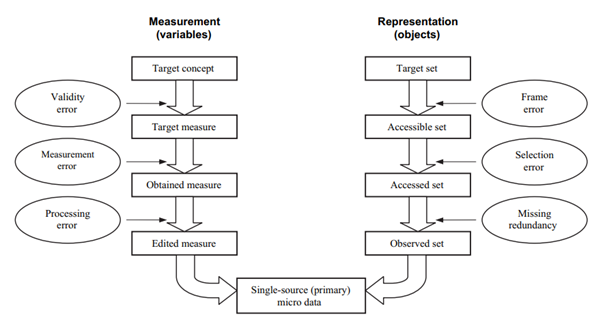
\includegraphics[scale=0.9]{ZHANG2012.png}
    \caption{Single-source data quality assessment framework \cite{ZhangTSE2012}}
    \label{fig:zhang}
\end{figure}

\subsection{Review of commonly-used approaches}
 Errors can be estimated and corrected by numerous methods. In this section we discuss some of those methods for single-source data and multiple-source data with one error source. We limit our research to errors in categorical variables, so-called classification errors. 

\subsubsection{Single-source data}
\\Firstly, we discuss correction method for errors on the right side of the quality assessment framework. Frame errors, mostly referred to as coverage errors, can be corrected with capture-recapture methods \shortcite{capturepopulation2015}. Selection errors, called sampling errors in the context of surveys, leading to unit non response are often corrected with weighting methods \shortcite{nonresponsebook2011}. Item nonresponse with (multiple) imputation methods \cite{handbookflexibleimputation_buuren2012}. 
\\ Now, the errors on the left side of the quality assessment framework. Validity errors are mainly a conceptual problem and cannot easily be adjusted with statistical methods. Other measurement errors are often localised by looking at impossible combinations with other variables, and corrected with minimal adjustments, based on the Fellegi-Holt paradigm, to comply with edit rules. For more information on statistical data editing we refer to the work of \shortciteA{handbookdataediting2011}. 

\subsubsection{Multiple-source data}
\\ Instead of using one source of data, using multiple sources creates more opportunities for error detection and correction. Conveniently, NSIs are often able to link variables from different sources on the unit-level together in a combined dataset. An important method that makes uses of multiple data sources is the latent variable modelling (LVM) approach; e.g. see \citeA{BiemerLCA}. LVM, with latent class (LC) analysis used specifically for categorical variables, uses multiple measurements of the same phenomenon \cite{Oberski2017LC}. Those measurements, either from the same source over time or from several sources at the same time-point, are then used as the ‘indicators’ of a latent, unobserved, ‘true’ score of the target phenomenon. An advantage is that, in contrast to alternative methods to correct errors, there is no need for error-free validation data. LVM assumes that none of the indicator variables of the sources are error-free, which is a more realistic assumption. For data measured over time, Hidden-Markov Models (HMM), a special case of LVM, can be used \shortcite{PavlopoulosVermunt2015, pankowska_measurement_2020}. For data from several sources at the same time-point, the Multiple Imputation of Latent classes (MILC) method can be used. MILC is developed by \shortciteA{boeschoten_etal2017MILC} and combines a LC model to estimate the errors with multiple imputation, to also correct the estimands for those errors. MILC is the main focus of this thesis and will be explained in section \ref{methods}.

\subsection{Situations with multiple errors} \label{energyexample}
Before explaining the methods, we will first explain the problem addressed in this study with an example situation. It concerns the production of statistics per subgroup based on data where the division of the groups is not the same for the each variable in a combined dataset. In this situation two sources of errors, selection and measurement error, can both be encountered. 
For the production of energy usage statistics, NSIs receive information about energy usage per address from multiple energy suppliers. To make meaningful statistics per subgroup they need to know whether each building is used for living or that it has a business function; whether it is a dwelling or an establishment. Additionally, NSIs are interested in the sector the businesses are active in. This information is not always supplied or even known by the energy provider, but can be matched with a register of the Chamber of Commerce. Herein all businesses are registered and their address and business activity recorded. However, some information is outdated, or simply wrong, which results in biased statistics.

\\When a business is registered at an address but performs its business elsewhere or e.g. online, such that the energy use of the building should be attributed to ``living" and not to business activities, this can be classified as selection error; units are wrongfully classified as establishments instead of dwellings and the dataset contains more objects than desired. Especially error-prone is the division of units into subgroups regarding their business activity or location. It can happen that a business moved or stopped without timely reporting it. Additionally, a business can be active in multiple regions or multiple business sectors introducing ambiguity and measurement errors. So when producing for example a statistic on the energy use per sector or per region based on a combined dataset with addresses, selection and measurement errors can occur simultaneously. This example situation will be used to guide the reader in the remainder of this thesis.

\\Selection error is from the representation side, and measurement error from the measurement side of the quality assessment framework (see figure \ref{fig:zhang}). While the total error frameworks provide a foundation for explicit decomposition of errors, it has been more successfully used as an intellectual framework than as a statistical model for error measurement \cite{Groves2010TotalSE}. The interplay of different error sources remains an under-researched area. It has also not been researched extensively whether existing methods are applicable in situations where misclassifications can be identified as being caused by different error types. In survey research there is an approach for multiple types of measurement errors, the multitrait-multimethod (MTMM) approach \shortcite{MTMM2015}. It is used for studying systematic, caused by survey design, and random measurement error simultaneously using experiments. However, this method targets variables measuring multiple concepts, while the variables in the combined datasets we are interested in, measure the same concept. MILC is used for estimating measurement error in combined datasets but has not been tested for its applicability to estimate multiple errors simultaneously. The focus of this research is on assessing the usefulness of MILC and its adaptation tree-MILC for situations with multiple error types.

\section{Methods}\label{methods}
In this section, the two methods under investigation, MILC and its adaption, tree-MILC, will be explained and compared. Both methods are used on combined datasets with unit-linked categorical variables measuring the same concept with the goal of calculating consistent statistics.

\subsection{MILC}
The MILC method, developed by \shortciteA{boeschoten_etal2017MILC}, is used to identify and correct classification errors in combined datasets. MILC is a combination of LC analysis (see e.g. Vermunt et al. 2008) and multiple imputation (MI) (see Rubin 1987). 

\\The typical use of latent variable models is for analysing multivariate response data with the goal of distributing units of the dataset over LCs. The number of LCs of a model is usually determined by comparing their model fit. In contrast, the LC model in MILC is used to estimate the “true” category of units in combined datasets, so the number of LCs is usually the number of categories of the indicator variables. While MI is typically used for missing data, in MILC multiple imputation is used to impute the correct class for all observations.

\\The MILC method consists of five MILC steps as can also be seen in figure \ref{fig:MILC}. In the remainder of this methods section, each step will be explained separately.

\newpage
\begin{figure}[h]
    \centering
    \includegraphics[scale=0.6]{MILC n.png}
    \caption{Graphical overview of the MILC method. At step 1 \textit{M} bootstrap samples are taken from a dataset containing multiple indicator variables. At step 2 a LC model is applied to each bootstrap sample and probabilities (denoted with $\pi$) are obtained. At step 3 \textit{M} imputations (denoted with the vertical bar) for the latent variable are created and placed next to the dataset. At step 4 the estimates of interest (denoted with $\theta$) are calculated from the imputations. At step 5 the estimates are pooled.}
    \label{fig:MILC}
\end{figure}

\textit{\textbf{Steps of MILC method}
}\begin{enumerate}
\item Take \textit{M} bootstrap samples with replacement from a dataset with unit-linked categorical variables from different sources measuring the same attribute, with \textit{M} being equal to the number of imputations (see step 3).
\item	Apply a LC model with \textit{C} classes on each of these \textit{M} bootstrap samples, with \textit{C} being equal to the number of categories of the variable of interest. 
\item	Sample from the obtained posterior membership probabilities to create \textit{M} imputations of the latent classes and store them in a dataset with the original variables.
\item	Calculate the estimate of interest $\hat{\theta}$ for each of the \textit{M} imputations
\item	Pool the \textit{M} estimates with Rubin’s pooling rules
\end{enumerate}



\subsubsection{Bootstrap step}
By taking non-parametric bootstrap samples from the original combined dataset we are able to reflect parameter uncertainty in the later steps of the MILC method. Without reflecting parameter uncertainty the variance of the estimates cannot be validly estimated. The bootstrapping is done by sampling with replacement from units in the combined dataset. This step results in \textit{M} bootstrap samples of the same size as the original dataset, with \textit{M} being the number of imputations we want to create in step 3. 

\subsubsection{Latent Class Model}
On each of the \textit{M} bootstrap samples we apply a LC model. The basic idea behind latent class analysis (LCA) is to find latent variables based on the correlation structure of observed categorical “indicator” variables. Each of the \textit{V} categorical variables has $C_v$ possible outcomes for each of the \textit{N} individuals. In our specific case, each source measures the same attribute and has the same number of categories, so $C_v = C$. Each individual has a response on each of the \t the {V} variables $Y_v \left(v=1,\ldots,V\right)$; for now we consider a situation without missing data. 
The vector of responses \textbf{Y} for one individual is called a response pattern. There are $\prod_{v=1}^{V}C_v\ $, and in our case $C^V$ possible response patterns. In LC theory, the number of LCs is not known and has to be determined by the user of the LC model. When a LC model is used for correction of classification errors, the number of LCs is fixed to \textit{C}, the number of categories in the variable of interest. 


The two key model assumptions for LC analysis are the local independence assumption and the mixture assumption. By assuming that responses within one LC \textit{X} are independent of each other, we assume the correlation between them was solely caused by their class membership. With this assumption we can calculate the likelihood of a response pattern \textbf{Y} occurring given the observation is part of class \textit{C}:

\begin{equation}
  P\left({\textbf{Y}}|X=c\right)=\prod_{v=1}^{V}P\left(Y_v|X=c\right)
\end{equation}
By assuming that the probability of obtaining a specific response pattern is the weighted sum of all \textit{C} class-specific conditional response probabilities (mixture assumption) we can express the probability density function of a response pattern \textbf{Y} across all classes:  
 
 \begin{equation}
P\left({\textbf{Y}}\right)=\sum_{c=1}^{C}P\left(X=c\right)P\left({\textbf{Y}}|X=c\right)	
 \end{equation}
By combining the mixture and local independence assumption and using Bayes’ rule, we are able to calculate the posterior membership probabilities of each response pattern, and thus for each unit in the dataset. The following holds:
\begin{equation}
 P\left(X=c |{\textbf{Y}}=
 {\textbf{y}}\right)=\frac{P\left(X=c\right)P\left({\textbf{Y}}={\textbf{y}}|X=c\right)}{P\left({\textbf{Y}}={\textbf{y}}\right)}    
\end{equation}



\subsubsection{Multiple Imputation}
While multiple imputation is typically used for imputing missing data, it can also be used to impute all values. This is the case in MILC \shortcite{boeschoten_etal2017MILC}, but also in overimputation \shortcite{blackwell_OI_2017}; for a comparison, see the work of \citeA{ Liu2020}. 
In MILC, MI is used for the imputation of all classes based on the results of the LC models as clarified below. See \shortciteA{VidottoVermunt_LC_MI2015} for an overview of other uses of LC models for imputation. 

In general, there are multiple methods to assign individuals to classes based on the posterior membership probabilities; see for an overview \citeA{bakk2015contributions}. The most straightforward method to impute the classes with the posteriors is modal assignment: individuals are assigned to the class with the highest posterior membership probability based on their response pattern. In MILC, a stochastic (proportional) assignment is used; values are assigned to a class by sampling from the posterior membership probabilities obtained by the LC step. We create \textit{M} empty variables and impute them with one of the classes by sampling from the posteriors of each of the \textit{M} bootstrap samples. Five imputations are usually sufficient, as demonstrated by \shortciteA{boeschoten_etal2017MILC}. 
 
 
\subsubsection{Calculation of estimates}
The goal of MILC is to produce consistent and unbiased statistics. We are interested in the sizes of the LCs and in the relation between the LC and the covariate. For the categorical variables of interest we can calculate the proportions of their frequency distributions. Since both the covariate and the LC in our simulation study are categorical, the relation between them is presented in a cross-table. We are thus interested in two types of estimates. Firstly, the sizes of the LCs, calculated as the proportion of units assigned to each class. Secondly, the relation between the covariate and the LC, calculated as the marginal proportion of units in each cell of the cross-table between them. We calculate these estimates for each of the \textit{M} imputations, which results in \textit{M} estimates. 


\subsubsection{Pooling of estimates} \label{Poolingrules}
We pool the estimates of the imputations with the standard pooling rules for imputation: Rubin’s pooling rules \cite{Rubin1987}. 
The pooled proportions are obtained by calculating the mean of the proportions over all \textit{M} imputations:
\begin{equation}
    {\overline{\theta}}=\frac{1}{M}\sum_{m=1}^{M}{\hat{\theta}}_m.						
\end{equation}
The total variance of the estimate is calculated by adding the within variance to a weighted between variance:		
\begin{align}
    V_{T}={\overline{V_{W}}+\left(1+\frac{1}{M}\right){V}_{B}}.
\label{eq:totalvar}
\end{align} 				
The pooled within variance is the average of the variance of each estimate and can be expressed as	 
\begin{equation}\label{withinvariance}
    {\overline{V_{W}}}=   
        \frac{1}{M}\sum_{m=1}^{M} Var(\hat\theta_m)=
    \frac{1}{M}\sum_{m=1}^{M} \frac{\hat\theta_m (1-\hat\theta_m)}{N} ,
\end{equation}				
with \textit{N} being the sample size of the combined dataset.
\\The between variance is the variance between the imputations which gives us:
\begin{equation}
    {V}_{B}=\frac{1}{M-1}\sum_{m=1}^{M}
    {({{\hat\theta}}_m-{\overline{\theta}})}^2.	
\end{equation} 		
The variance due to the bootstrapping is reflected in the between variance. As a result, the total variance of the estimates can be validly estimated. Its square root, the standard deviation $sd$ can be used to construct the confidence interval around $\overline{\theta}$ in the following manner: 

\begin{equation} \label{EQconfidenceinterval}
    \overline{\theta} \pm  z_{0.975}* sd.
\end{equation}	

\subsection{Tree-MILC}
Tree-MILC is potentially a useful method to obtain consistent estimates for combined datasets containing errors of multiple types. The tree part of the method is specifically applicable on variables that have a subgroup structure. This is the case in the energy statistic example introduced in section \ref{energyexample}, the units in the dataset are split into dwellings and establishments, of which the latter are divided into three subgroups, e.g. business sectors. As this demonstrates, the application of tree-MILC is very dependent on the (subgroup) structure of the variables and the sources of errors in the data. 

\\The idea of implementing a tree-step, and naming the method tree-MILC, originates from latent class tree (LCT) analysis, as developed by \citeA{bergh2018latent}. In LCT analysis, the data is split and structured into classes by method of a sequential comparison of 1- and 2-class models. The top-down approach continues until the information criterion (e.g. BIC) no longer chooses 2-class models over 1-class models. The splits are performed based on the posterior class membership probabilities of each new class (child nodes) conditional on the class before the splitting (parent node). The advantages of this method of LC analysis are that it provides clear insight in splitting of the classes and the structure of the data, and on how models with different number of classes are related to each other. A schematic overview of a LCT analysis can be seen in figure \ref{fig:LCTmattis}.

\begin{figure}[h]
    \centering
    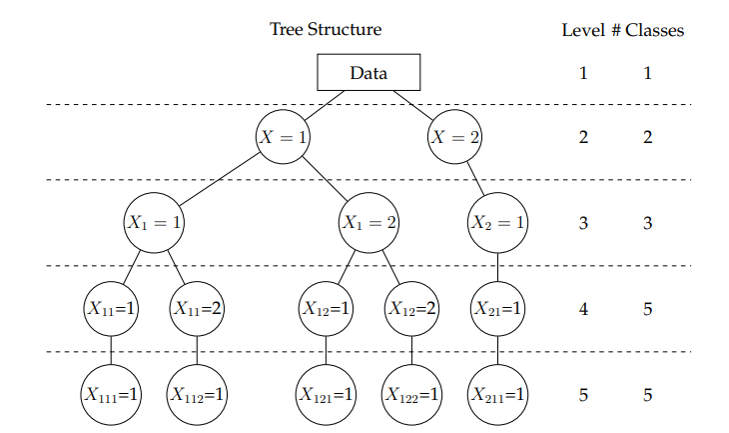
\includegraphics[scale=.6]{LCTmattis.png}
    \caption{Schematic overview of a latent class tree analysis \cite{bergh2018latent}}
    \label{fig:LCTmattis}
\end{figure}

LCT analysis is an exploratory method with a main purpose of helping determining the number of classes. In our situation the number of classes is fixed and dependent on the categories of the variable. Therefore we do not use the LCT as intended, but we only use the idea of a tree-structure to distinguish between the two sources of errors and apply a LC model twice. 

\\Tree-MILC has the same procedure as MILC, with an extra LC model and MI step before the estimates are calculated. We name the first LC and MI step ``selection error phase" and the second LC and MI step the ``measurement error phase", as visible in figure \ref{fig:treeMILC}. The first LC model and MI step are applied on the whole dataset to estimate the selection errors. In light of the energy statistic example this can be viewed as the stage where the units are classified as a dwelling or an establishment. Based on the imputations from the selection error phase, we take subsets from each bootstrapped dataset, to end up with a ``child node" with only the selected cases. In our example, the subsets with the selected cases contain all the establishments. In the measurement error phase, the LC model and MI step are applied on the subsets to estimate the classification errors. In the energy statistic situation this could represent the errors regarding the classification of the units in businesses sectors. After both error phases, the imputations of both are combined, and estimates are pooled with Rubin's pooling rules (see section \ref{Poolingrules}). An overview of the tree-MILC steps can be seen in figure \ref{fig:treeMILC}. Both phases will be explained in more detail in the next two subsections.
\begin{figure}[h]
    \centering
    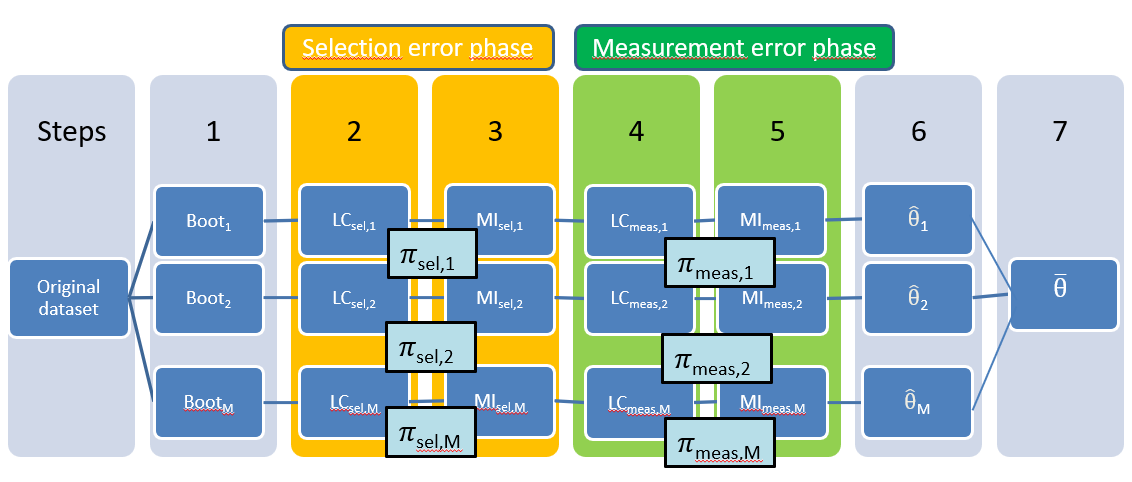
\includegraphics[scale=.7]{TreeMILCprocess9mei.png}
    \caption{Schematic overview of steps of tree-MILC: 
    At step 1, \textit{M} bootstrap samples are taken from a dataset containing multiple indicator variables. At step 2, a LC model is applied to each bootstrap sample and posterior probabilities (denoted by $\pi_{sel}$) are obtained. With the imputations calculated in step 3, subsets are created to which the LC model in step 4 is applied. At step 5 imputations are calculated for the subset using the obtained posterior probabilities (denoted by $\pi_{meas}$). The imputations of the subset replace the imputations of the entire dataset from step 3 where appropriate. At step 6 estimates of interest (denoted with $\hat\theta$) are calculated for the dataset   with the combined imputations of both phases. At step 7 the estimates are pooled.} 
    \label{fig:treeMILC}
    %
    % 
\end{figure}
\subsubsection{Selection error phase}
After the \textit{M} bootstrap samples are taken from a combined dataset containing multiple indicator variables, which is done in exactly the same way as in MILC, the selection error phase begins. A LC model is applied with \textit{S} classes to estimate the selection errors, with \textit{S} being the number of subgroups of interest in the categories of the variables in the combined dataset. By sampling from the obtained posterior membership probabilities from the \textit{M} LC models, all cases are assigned to one of the \textit{S} classes. The \textit{M} imputations are placed in \textit{M} columns next to the original dataset. Based on those imputations we create a subset for each of the bootstrap samples that contain the cases of our target set. This subset is used in the next phase.

\subsubsection{Measurement error phase}
 The measurement error phase is applied on each of the \textit{M} subsets created in the selection error phase. We start by applying a LC model with \textit{C} classes to each of the bootstrap samples, with \textit{C} being the categories prone to measurement error. We then impute the classes by sampling from the obtained posterior membership probabilities. The \textit{M} imputations of the measurement error phase are replacing the imputations from the selection error phase where applicable. This is possible since the imputations in the measurement error phase are sub-categories or ``sub-classes'' of the ``selected'' class. This results in a dataframe with the original data, and next to it \textit{M} columns with imputed variables. The imputed latent variables have a total of $S-1+C$ categories; $S-1$ categories without further subdivision and $1$ category that can be split into $C$ categories. This total is equal to the number of categories in the original dataset. When the imputations of the selection and measurement error phases are combined, the estimates of interest (denoted with $\hat\theta$) are calculated. Lastly, the estimates are pooled with Rubin's pooling rules.

\section{Simulation study} \label{ch_simstudy}
To investigate the performance of the methods explained in section \ref{methods} in estimating and correcting for selection and measurement errors in combined datasets we performed a simulation study. For this study, we generated a large number of datasets with four variables on the same concept in which synthetic measurement and selection errors of several levels were introduced. We simulate a population with indicator variables and assign each unit to a LC. From this assignment of LCs we calculate the population estimates. Then we apply both MILC and tree-MILC on the same datasets, and calculate the pooled imputed estimates. 

By performing a simulation study, we are able to compare the estimates of MILC and tree-MILC against an objective population value. Another advantage of a simulation is that we can examine how the methods perform on datasets with different properties, by comparing the results of several simulation conditions. 

All computations for the simulation study were performed with statistical software R (v4.0.3) \cite{Rproject}. In particular, the R package \textit{poLCA} (v1.4.1) \cite{poLCA_package} will be used for the data generation and the estimation of the LC model. Instructions and reproducible scripts are available in the \href{https://github.com/daniellerem/Thesis-treeMILC}{research archive} of this study. Ethical approval from the University's ethics board was obtained. The simulation study consists of three parts which will be discussed in order: the data generation, the appliance of the MILC and tree-MILC methods, and the calculation of performance measures used for the evaluation of the results. Thereafter, expectations about the results of the simulation study are formulated.

\subsection{Dataset generation} \label{Dataset_generation}
We generated 1,000 populations of 5000 units and applied both methods to each of the generated populations. As a result, we perform the simulation $N_{sim}= 1000$ times, with $N_{sim}$ being the number of simulation iterations. The datasets we use consist of units from a theoretical population with a large sample size of $N=5000$, measured by five variables: four polytomous indicator variables (Y), each with four categories, measuring the latent variable (X), and one polytomous covariate (Z), again with four categories. The number of simulation iterations and the dataset's sample size are chosen to accelerate convergence of the LC model and of the simulation results. The \textit{poLCA} function we use to generate the data provides us with a ``true class" variable that represents the LC each unit belongs to in the ``real world''. We use the energy example for clarification: the generated true LC signifies what group (dwelling or an establishment in a specific sector) a unit belong to in reality, not what it is stated to be in a variable. This population value is in reality not always attainable, but is available in the simulation study. We calculate this value by averaging the proportions of each LC in the true class variable over all the generated datasets. In appendix \ref{Pop} the calculated population estimates can be found. 

The datasets are generated with the \textit{poLCA} package, which allows for specifications of a probability distribution that describes the relation of each indicator variable with respect to the latent variable. We assign four LCs to our population. The four LCs correspond with the four categories of the indicator variables, meaning that without any errors in the data all indicator variables should have the same category as the LC; the numbers should match. 
\begin{table}[hb]
\centering
\caption{Simulation conditions}
\hspace{3cm}
\begin{tabular}{lrllcccc}
\hline
&&&& \multicolumn{4}{c}{Measurement error}\\ \cline{5-8} 
&&&& \multicolumn{2}{c}{5\%} & \multicolumn{2}{c}{20\%} \\ \cline{5-8} 
&&&& \multicolumn{4}{c}{Covariate} \\ \cline{5-8} 
&&&& Weak      & Strong      & Weak       & Strong      \\ \hline
Selection error & 5\%  & Covariate & Weak   & - & 2 & - & 4 \\ \cline{4-8} 
&&& Strong & 1 & - & 3 & - \\ \cline{2-8} 
& 20\% & Covariate & Weak   & - & 6 & - & 8 \\ \cline{4-8} 
&&& Strong & 5 & - & 7 & - \\ \hline
\end{tabular}
\label{Tab:sim_conditions8}
\end{table}

To see how MILC and tree-MILC perform on datasets with different structures, we generated data with eight different variations on the described theoretical population. The simulation conditions differ by the level of selection error and the level of measurement error for the indicator variables and the source of error strongly associated with the covariate. 

The simulation study has been performed on simulated datasets with the following features. We have four indicator variables with four categories each, and one covariate with the same four categories. We vary the levels of selection error (5\% and 20\%) and classification error (5\% and 20\%). For each of the four combinations of selection and classification error, we also have two versions in which we vary the properties of the covariate. One version has a covariate that correlates strongly with selection error, the other has a covariate that correlates strongly with measurement error. This totals to eight simulation conditions, which are depicted in table \ref{Tab:sim_conditions8}.

The datasets are generated using the following procedure. In a first dataset with four indicators variables and one covariate that contain the selection errors, we assign two LCs with $P(1)=0.15$ and $P(2)=0.85$. The errors are specified in the probability distribution that describes the relation of each indicator variable with respect to the latent variable
See table \ref{tab:selectionerror} for the probability distribution of one indicator variable with selection error. The probability distributions of all indicator variables are specified identically. 

\begin{table}[t]
\centering
\caption{Selection error for one indicator variable, Y_i}\\
\vspace{1}
\begin{tabular}{l cc l  l cc}
 \hline
& \multicolumn{2}{c}{5\%} &&&  \multicolumn{2}{c}{20\%}  \\
  \cline{2-3}
  \cline{6-7}
 LC & P(Y_i=1) & P(Y_i=2)  &&&   P(Y_i=1) & P(Y_i=2)  \\ 
  \hline
 X=1  & 0.95 & 0.05 &&& 0.80 & 0.20  \\ 
  X=2 & 0.05 & 0.95 &&& 0.20 & 0.80  \\ 
  \hline
  \end{tabular}
  \label{tab:selectionerror}
\end{table}



\begin{table}[t]
\caption{Measurement error probabilities for indicator variable, $Y_i$}
\centering
\begin{tabular}{l ccc r ccc }
 \hline
   &  \multicolumn{3}{c}{5\%} && \multicolumn{3}{c}{20\%} \\
 \cline{2-4} 
 \cline{6-8}
 LC & P$(Y_i=1)$ & P$(Y_i=2)$ & P$(Y_i=3)$ &&  P$(Y_i=1)$ & P$(Y_i=2)$ & P$(Y_i=3)$\\ 
  \hline
  X=1 & 0.95 & 0.025 & 0.025 &&0.80 & 0.10 & 0.10\\ 
  X=2 & 0.025 & 0.95 & 0.025 &&0.10 & 0.80 & 0.10\\ 
  X=3 & 0.025 & 0.025 & 0.95 &&0.10 & 0.10 & 0.80 \\ 
  \hline
  \end{tabular}
  \label{tab:measurementerror}
\end{table}


In the second dataset, the four indicators variables and the covariate contain measurement errors, see table \ref{tab:measurementerror} for the probability distribution of one indicator variable conditional to the LC. We assign three LCs with theoretical probabilities of respectively 0.4, 0.35 and 0.25. We change the values of the imputed LCs by adding one ($+1$) to avoid conflicts when combining it with the first dataset. As a result, the simulated LCs 1, 2 and 3 are now called 2, 3, and 4. The next step is namely to replace all the cells associated with LC 2 in the first dataset with values from the second dataset we simulated. 


\begin{table}[bh]
\centering
\caption{Covariate relation with selection error}\\
\vspace{1}
\begin{tabular}{l cc l l cc}
 \hline
& \multicolumn{2}{c}{weak} &&&  \multicolumn{2}{c}{strong}  \\
\cline{2-3} 
\cline{6-7}
 LC & P(Z=1) & P(Z=2)  &&&   P(Z=1) & P(Z=2)  \\ 
  \hline
 X=1  & 0.5 & 0.5 &&& 0.70 & 0.30  \\ 
  X=2 & 0.5 & 0.5 &&& 0.30 & 0.70  \\ 
  \hline
  \end{tabular}
  \label{tab:selectionerrorCOV}
\end{table}



\begin{table}[h]
\caption{Covariate relation with measurement error}
\centering
\begin{tabular}{l ccc r rrr }
 \hline
  &  \multicolumn{3}{c}{weak} && \multicolumn{3}{c}{strong} \\
\cline{2-4} 
\cline{6-8}  
 LC & P(Z=1) & P(Z=2) & P(Z=3) &&  P(Z=1) & P(Z=2) & P(Z=3)\\ 
  \hline
  X=1 & 1/3 & 1/3 &1/3 &&0.70 & 0.15 & 0.15 \\ 
  X=2 &  1/3 & 1/3 &1/3 &&0.15 & 0.70 & 0.15 \\ 
  X=3 &  1/3 & 1/3 &1/3 &&0.15 & 0.15 & 0.70 \\ 
  \hline
  \end{tabular}
    \label{tab:measurementerrorCOV}
\end{table}
This process results in a dataframe with four indicator variables with four categories each, and one covariate with four categories. The four LCs theoretically have the following population probabilities: 0.15, 0.34, 0.2975, and 0.2125. The three latter values are calculated by multiplying the probability of LC 2 in the first dataset with the probabilities of the LCs in the second dataset, e.g. $0.85*0.4=0.34$. In practice, the class sizes differ slightly per condition, as visible in Appendix \ref{Pop}. With the replacement step in the data generation procedure, a tree-like structure is given to the LCs. %as can be seen in figure \ref{fig:LCpopulation}.

The covariates are simulated using a similar procedure as for the indicator variables, but their purpose is different. In each of the conditions, the covariate either has a strong relation with selection error, or a strong relation with measurement error (see tables \ref{tab:selectionerrorCOV} and \ref{tab:measurementerrorCOV}). In practice the former means that the covariate is correlated strongly with LC 1, and the latter that the covariate is correlated strongly with classes 2, 3 and 4.


%\begin{figure}[h]
%    \centering
%    \includegraphics[scale=.5]{LCprobs.png}
%    \caption{Theoretical marginal population probabilities of the latent classes}
%    \label{fig:LCpopulation}
%\end{figure}

\subsection{Application of MILC and tree-MILC}
The MILC and tree-MILC methods are applied on the same data. Results of both methods for each simulation condition are presented and compared in the results section. 

As explained in the methods section, we start with taking \textit{M} bootstraps of each generated dataset using the frequency patterns of each response pattern. On this data we apply a LC model with the indicator variables and the covariate. We include the covariate in the LC model since all variables in whose relation with the LC you are interested in should be added. The number of classes in the LC model for MILC is four. The number of classes in the LC model for tree-MILC is two in the selection error part, and three in the measurement error part. 

An important technicality to note about the application of the LC models is the label switching problem. The essence of the problem is that the likelihood of LC models is invariant with respect to permutations of the component labels; the labels of the LCs are arbitrary to the model. Since we are interested in comparing the size of the classes over multiple iterations of the model by taking the average value, the labels are crucial for the evaluation. To solve this label switching problem we use a concept called ``column maxima switched label detection" (Tueller, 2011). We sort the order of the classes in the conditional probabilities column-wise by their maximum probabilities, such that the highest probabilities are placed in the diagonal entries of the matrices with posterior membership probabilities. Subsequently we use \textit{poLCA} functions to reorder the LC results with the right labels. With the obtained \textit{poLCA} object we can calculate the posterior membership probabilities, with which we draw the corresponding \textit{M} imputations. 

\subsection{Evaluation criteria}
When evaluating the performance of MILC and tree-MILC, we are interested in whether the imputed latent variable has similar properties as the simulated true latent variable. Therefore, we inspect the size of the LCs; the pooled proportions of each class averaged over all the simulations. Also important is whether the relations between the latent variable and other variables are preserved. So secondly, the relationship of the LC with the covariate is investigated. This is done by comparing the cross-table between the covariate and the imputed latent variable, with the cross-table between the covariate and the true latent variable. The latter cross table can be seen in appendix \ref{A_Table_Prop}.

Both properties, LC sizes and class-covariate relations, are assessed by calculating performance measures for each simulation condition, and averaging those results over the number of simulations. To investigate how similar the properties of the imputed variable of both methods are to the theoretical latent variable, we look at two measures of accuracy and two 95\% confidence interval measures. The four performance measures will be clarified in the two next sections.

\subsubsection{Accuracy performance measures}
To compare the accuracy of the results, two measures are calculated from the absolute difference between the true estimate and the estimate obtained with the method. The first is the root mean squared error (RMSE) and the second is the mean absolute relative error (MARE). The main difference between the two accuracy criteria is that the RMSE is an absolute criterion and in the same scale as the estimate, while the MARE is a relative criterion. In the latter the estimates are divided by their population values as to reduce the effect of the estimate's size when comparing estimates of multiple sizes. 

This should not be confused with the fact that to calculate MARE, we take an absolute value of the relative difference. This is done to 

\\While the information about the direction of the (relative) difference between the true and obtained estimates is lost for both criteria, this is done to be able to make conclusions about the size of the differences. Because a bias measure that is low can wrongfully imply a good performance when the estimates deviate greatly from the true value but converge to zero on average.

The root mean squared error (RMSE) is an accuracy measure equal to the square root of the average squared deviation of the pooled estimate from the population value.

\begin{equation}
    {\text{RMSE}}=\sqrt{\cfrac{\mathlarger\sum_{s=1}^{N_{sim}}
    \bigg(\overline{\theta}_s-\theta\bigg)^2}
    {N_{sim}}} .
\end{equation}	

The mean absolute relative error (MARE) is an accuracy measure equal to the average of the
absolute deviation of the pooled estimate from the population value divided by the population value.

    \begin{equation}
     \text{MARE} =  \frac{\mathlarger\sum\limits_{s=1}^{N_{sim}}\bigg | {\cfrac{\overline{\theta}_{s} - \theta}{\theta}\bigg |}}{{N_{sim}}}.
     \end{equation}
 The calculation of the relative error is chosen as to reduce the impact of the class size on the error and to be able to compare the error between classes independent of their sizes. 




\subsubsection{confidence interval performance measures}
We want to investigate whether the results of the simulation study fall in the expected range of values based on the population estimates and how precise the estimates are. For this end we use two performance measures: the coverage of the 95\% confidence interval (CI) of the population estimate, and the average width of the 95\% CIs of each simulation iteration. The limits of the 95\% CI around the estimate of interest of each simulation iteration $s$ is calculated with the upper confidence limit
\begin{equation}
    {\text{UCL}_s} = \overline{\theta}_s + z_{0.975}* sd_s,
\end{equation}
and the lower confidence limit
\begin{equation}
    \text{LCL}_s = \overline{\theta}_s - z_{0.975}* sd_s.
\end{equation}
The standard deviation, $sd$, is the square root of the total variance ($V_T$, see equation \ref{eq:totalvar}). 
The 95\% confidence interval width is the difference between the upper- and the lower limit of the CI, averaged over the number of simulations:
\begin{equation}
  \frac{ \mathlarger\sum^{Nsim}_{s=1} 
   \bigg(\text{LCL}_s - \text{UCL}_s\bigg)}
   {N_{sim}}.
\end{equation}

The empirical coverage probability of the 95\% confidence interval is equal to the proportion of simulated results whose 95\% confidence interval, constructed around the simulated estimate, contains the true population parameter. The coverage of the 95\% CI is defined as following:
\begin{equation}
   P( \text{LCL}_s \leq{\theta} \leq \text{UCL}_s) = \frac{ \mathlarger\sum^{Nsim}_{s=1} \bigg(\Bigg{\text{I}_{s}}\bigg)}
   {N_{sim}},
\end{equation}
with the indicator function giving a ``1'' when the population estimate falls within the confidence interval of the sample estimate, and a ``0'' when not:

\[ \text{I}_{s}= \begin{cases} 
      0 & \theta < \text{LCL}_s\\
      1 & \text{LCL}_s \leq \theta \leq \text{UCL}_s \\
      0 & \text{LCL}_s< \theta .
   \end{cases}
\]

\subsection{Expectations}
We expect the more complex tree-MILC method to perform better than MILC with respect to calculating the estimates. Good performance involves high accuracy, good coverage of the 95\% CI, and a low variance. These properties can be demonstrated with a low MARE and RMSE for high accuracy, a coverage between 93\% and 97\% for good coverage, and small 95\% CI widths for low variance. 

\\For all estimates, we expect the methods to perform worse on datasets with higher errors than on datasets with lower errors. The performance of the methods is expected to be influenced by the levels and sources of errors in the simulated data as specified in the conditions, and by the class sizes. We refer back to table \ref{Tab:sim_conditions8} and the data generation section (section \ref{Dataset_generation}) for an overview of the specifications of all conditions. In the remainder of this section we outline the expectations we have for the two types of estimates.

In the conditions with small selection error (5\%) we expect a good performance of both methods. Within the four conditions with small selection error, the conditions with high measurement error (20\%) are expected to have a lower performance on the classes affected by measurement error, which are classes 2, 3, and 4, than the conditions with low measurement error. As tree-MILC is designed to target the errors subsequently, we expect tree-MILC to perform better than MILC for the two conditions, numbered 3 and 4, with small selection error and high measurement error.

In the four conditions with high selection error we expect an overall worse performance of both methods than for the previously discussed four conditions with low selection error. However, we do expect tree-MILC to perform better than MILC. Especially for the conditions with high measurement error. We expect class 1 to be the most affected by selection error. So in conditions 5 and 6 we expect class 1 to have the relative worst performance among the classes, which can be compared with the MARE criterion. Conditions 7 and 8, with high levels of errors for both error sources, are considered to be the most `difficult' of all eight conditions. We therefore expect a bad performance for each class, but even worse for class 2, 3 and 4 because they are fully affected by both errors and class 1 is mostly affected by selection error.

One other expectation about the class size estimates relates to the source of error the covariate strongly correlates with. The conditions with a covariate that is strongly correlated to selection error (odd conditions) are expected to help with the classifications of the classes related to selection error (class 1 versus the others). The conditions with a covariate that is strongly correlated to measurement error (even conditions) are expected to help with the classification of class 2, 3, and 4. As a result of those two expectations, we expect to see both methods perform slightly better on classes 2, 3, and 4 in even conditions with high measurement error. Additionally, we expect to see tree-MILC in specific to perform better in odd conditions than in even conditions. 

The 95\% CI width of each estimate is affected by the total variation in the estimates. Estimates in more difficult conditions are expected to have larger variances. The 95\% CI is also dependent on the size of the estimate itself. Relatively larger estimates have relatively larger variances, which means that they have wider confidence intervals. As a consequence larger estimates have a higher probability of being covered in their confidence interval based on the 95\% CI width. 

Now we will briefly discuss some expectations specific for the covariate-class relations depicted in cross-tables between the covariate and the LC. The main question is whether the relationship between the covariate and the LC remains the same. We expect conditions on which the methods did not perform well for the class sizes, to also have a bad performance for the estimates in the cross-table. In specific, we expect cells in the class-covariate cross-table associated with the classes on which the methods did not perform well to also have a worse performance.

 %Whether the covariate has a strong relationship with selection or measurement error is also expected to be of importance. We expect in the former case (odd conditions) that ,  ... and in the latter case (even conditions) that 


To sum up, we have the following hypotheses about the results of the simulation study: 
\begin{enumerate}
    \item Both methods perform worse on datasets with higher errors 
    \item Tree-MILC has a better performance overall
    \item Class 1, and the relations between the covariate and class 1, are the most affected by high selection errors. Resulting in relatively better performances of both methods for the affected classes in the odd conditions than in the even conditions.
    \item Classes 2, 3, and 4, and their relationships with the covariate, are most affected by measurement error. Resulting in better performances of tree-MILC than MILC for the even conditions.
\end{enumerate}


\section{Results} \label{ch_results}
Some of the results of the simulation study are presented in graphs in this section to highlight notable results and simplify the discussion of the results. The complete simulation results are presented in tables \ref{A_Table_Prop} \ref{COVaccuracyresults}, and \ref{COVresultsCI} in appendix \ref{AppendixTables}. 

\begin{figure}[h]
    \centering
    \includegraphics[scale=0.5]{Boxplot_classes.png}
     \caption{Boxplots of relative absolute bias of class sizes (grey rows on the right) per method for eighth conditions (columns) with $N_{Sim} = 1000$}
     \label{fig:boxplotrelbias}
\end{figure}


\subsection{Latent class sizes}
A first impression of the results for the class sizes can be seen in figure \ref{fig:boxplotrelbias}. In these boxplots the absolute relative errors of the results for each class are depicted. By averaging these values over the number of simulation iterations the MARE measure can be obtained. In the boxplot you can see an overview of the deviation and the spread of the results for the class sizes per simulation condition for both methods. The first impressions from the boxplot are the following: for low selection errors both methods perform equally well, for high selection errors tree-MILC performs better. Class 1 seems to be the class most affected by higher errors; both methods perform worse on class 1 than on the other classes in most conditions. The spread of the results for class 1 is larger than that of the other classes, there is more uncertainty, especially for more challenging conditions. 

The performance on the first four conditions on the LC sizes is similar for both methods. Both perform well; their accuracy is high, they have nominal coverage rates and small 95\% CIs. Within these four conditions, the only difference between the conditions with small and high measurement error seems to be the width of their 95\% CIs. For the classes affected by measurement error, the width is larger for conditions with high measurement error. 

In the last four conditions, with high selection error and varying levels of measurement error, the overall performance of MILC is worse. Especially for class 1, the class most affected by selection error. The performance of tree-MILC is only slightly worse, mostly visible for the performance of class 1: the coverage rates are slightly lower (around 90\%) than nominal, despite the wider 95\% CIs. Two observations regarding the performance of MILC alone are remarkable. Firstly, something we did not expect is MILC performing worse on conditions 5 and 6 than on conditions 7 and 8, while we designed the latter conditions to be the most challenging. Secondly, regarding the influence of the covariate on MILC's performance to predict the LC sizes: MILC seems to perform less bad on condition 5 than on 6, and less bad on condition 7 than on 8. The covariate correlated strongly with selection error in the odd conditions seems to improve MILC's performance for the class 1, the class associated with selection error. For the classes associated with measurement error, a similar effect has not been observed.

\begin{figure}[h]
    \centering
    \includegraphics[scale=0.5]{coverage_prop.png}
     \caption{Coverage of the 95\% CI of the class sizes (columns) for the eight conditions (rows) for both conditions (top) with $N_{Sim} = 1000$. The target coverage is 95\%.} 
     \label{fig:coverageprop}
\end{figure}
\begin{figure}[h]
    \centering 
    \includegraphics[scale=0.5]{coverage_covar.png}
     \caption{Coverage of the 95\% CI of the cross-table between classes (columns, below) and covariate (rows, left). Depicted for both methods (grey columns, top) and for eight conditions (grey rows, right) with $N_{Sim} = 1000$. The target coverage is 95\%.}
     \label{fig:coveragecovar}
\end{figure}

\subsection{Cross-table between LC and covariate}
The performance on the first four conditions on the cross-table is similar for both methods. Both methods perform well; their accuracy is high, they have nominal coverage rates and small 95\% CIs. No clear distinctions can be made between the conditions with a covariate correlating strongly with selection or measurement error.

In the four conditions with high selection errors, the accuracy is lower than for the conditions with low selection errors. The accuracy of MILC is lower than that of tree-MILC. The coverage rates of the 95\% CIs are nominal for both methods. It seems that the relation between the LC and the covariate has been preserved well, despite the errors in the datasets. 

\begin{figure}[h]
    \centering
    \includegraphics[scale=0.45]{Bias_covarSCALED.png}
     \caption{Mean absolute Relative Error (MARE) of cross-table between the LCs (columns, below) and covariate (rows, left). Depicted for both methods (grey columns, top) and for eight conditions (grey rows, right) with $N_{Sim} = 1000$. The darker the color, the higher the higher the MARE.}
     \label{fig:biascovar}

   \includegraphics[scale=0.5]{rmse_covarSCALE.png}
    \caption{Root mean squared error (RMSE) of cross-table between the LC (columns, below) and covariate (rows, left).  Depicted for both methods (grey columns, top) and for eight conditions (grey rows, right) with $N_{Sim} = 1000$. The darker the color, the higher the RMSE.}
    \label{fig:rmsecovar}
\end{figure}

%Overall, tree-MILC is better at covering the 95\% CI. The confidence interval widths are mainly used as a check to see if there are no abnormal small or wide intervals. This is not the case. However, it is noteworthy/remarkable that the confidence intervals get wider by increasing the conditions. Following, the results for the coverage of the 95\% CI for both types of estimates are discussed.
\subsection{Combined conclusions}
As expected, both methods performed better on conditions with low selection error than on the conditions with high selection error, and tree-MILC performed better overall. Specifically the class that is most affected by selection error, class 1, and the relations between class 1 and the covariate were more often predicted with higher deviations from the population value. Especially for the conditions with high selection error, and for the estimates most affected by selection error, tree-MILC does perform better than MILC. 

Despite classes 2, 3, and 4 all being exposed to the same amount of errors, we choose to depict all three, and not just one, to be able to see influence of their different sizes.
The results are very similar, but interesting to note are the differences between the RMSE and the MARE for the estimates. Where the RMSE of one estimate is higher than of the other estimates, its relative deviation as calculated by the MARE can be lower than of the other estimates. Another argument for the choice for MARE is that a relative measure makes a comparison between size of the errors for the LCs and the cross-table possible, despite the two types of estimates being on a different scale. Thus for unequal sized estimates, the MARE is a more comparable accuracy measure. 


%For the LC estimates, the accuracy measures follows the same pattern as the coverage rates; a lower accuracy corresponds to a lower coverage rate. For the covariates this pattern is not visible, because the values are in a lower scale, the deviations from the population value for the cross-table are much lower than for the LCs. 

%We accounted for the class sizes by calculating the relative bias. Almost without exception, within each condition, the bias is the highest for the smallest class, and the lowest for the largest class. From visual inspection of the boxplots, the spread seems to follow the same relation: the spread is the highest for the smallest class, and the lowest for the biggest class. 



\begin{figure}[h]
    \centering
    \includegraphics[scale=0.4]{ciwidth_prop.png}
     \caption{Average width of the 95\% CI of the class sizes (columns) for the eight conditions (rows) for both conditions (top) with $N_{Sim} = 1000$. The darker the color, the wider the 95\% CI.}
     \label{fig:ciwidthprop}
\end{figure}

\begin{figure}[h]
    \centering
    \includegraphics[scale=0.5]{ciwidth_covar.png}
     \caption{Average width of the 95\% CI of the cross-table between classes (columns, below) and covariate (rows, left). Depicted for both methods (grey columns, top) and for eight conditions (grey rows, right) with $N_{Sim} = 1000$. The darker the color, the wider the 95\% CI.}
     \label{fig:ciwidthcovar}
\end{figure}

\section{Discussion}
As described in section \ref{background}, consistent estimates can be obtained with the MILC method for combined datasts. An important requirement is that the variables in a unit-linked combined dataset measure the same concept. In this study we investigated the suitability of MILC and the adaptation tree-MILC to obtain consistent estimates for combined datasets that contain multiple sources of errors. We are interested in its performance in situations where misclassifications can be identified as being caused by selection and measurement errors. 

With the aim of comparing the performance of MILC and tree-MILC to produce a consistent statistic, a simulation study was conducted. In the simulation study eight versions (with different levels of errors) of a combined dataset containing variables with four categories and four LCs, the eight simulation conditions, were analysed with MILC and tree-MILC. The obtained estimates for 1,000 simulation iterations were compared to the population estimates from the generated datasets. 

Overall, both methods perform comparably well when the errors in the combined dataset are small. As expected, MILC performs worse in terms of accuracy and the coverage of the 95\% CI on classes subjected to higher levels of errors. The performance of MILC is indeed related to the `difficulty' of the simulation condition. Different than expected is that conditions five and six were more challenging conditions for MILC than conditions seven and eight. Although the variation of its estimates is higher for the conditions with high selection error, tree-MILC does perform well in terms of accuracy and coverage of the 95\% CI. In these cases, tree-MILC is a good alternative to MILC. 

Concerning the covariates, more research is necessary to make firmer conclusions but a first impression is that a covariate correlated strongly with selection error improves MILC's performance.

A drawback of tree-MILC is that the method is more complex and that its computation time is even longer than that of MILC, at least twice as long. The computation time for one run with MILC takes 3.5 minutes, for one run with tree-MILC at least twice as long. Even when making use of multiple cores with parallel computing the code, a simulation study with $N_{sim} = 1000$ using both methods takes days to complete.

So while we expected that the methods would perform the worst on the conditions with the highest errors, this was not the case. One possible explanation for this difference is the fact that the selection and measurement errors and the classes are dependent on each other. In datasets with higher levels of errors, the response patterns are more varied than in datasets with lower levels of errors. Therefore the chance of getting imputed in a different LC than the true class is higher in the former. If this is the case for all LCs (instead of only LC1 as is the case with selection error), the chance of them getting assigned wrongly is higher which makes the chance of getting correct estimates on average higher. Important to remember is that we are only interested in the LC sizes on average, not in the correct assignment of individual cases. This dependency can intuitively be understood as a sort of``waterbed effect''; where a class is wrongly classified, it gets assigned to one of the other classes, it does not disappear. Since we only have four classes in our simulation study, there are limited options for the miscategorised classes to be classified in. And thus the relatively better performance of both methods on the conditions with the highest errors can potentially be explained. 

%In the \textit{poLCA} package's function to simulate data, we are able to specify the target population values of the classes and the probability distributions for the LCs for each indicator variable and covariate. 

To be able to focus on the performance of both methods on a variety of datasets, specified in the conditions, we chose to keep all other possible simulation parameters consistent at a level that will not cause any problems. An example is that the dataset has a sample size of $N=5000$, and four indicator variables. Both are relatively large, and possibly unrealistic, but contribute to the convergence of the LC model and allows us to focus on the differences in performance caused by the specifications of the errors. 

Further research should vary the height of both errors more dynamically, and study the interplay between the two errors. It is interesting to study the effect of the data generation mechanism on the performance further. The simulated data contains variables with four possible categories and thus four LCs. What if the data contains more categories? Does this influence the performance in a negative way? Another potential scenario that can resemble situations encountered in practice, are datasets where multiple subgroups can be categorised. Potentially the measurement error phase can be applied multiple times, at multiple subgroups, or even at subgroups within a subgroup. Does tree-MILC still work or does it get too complex and susceptible to errors? 

We now return to the problem we started with in order to give the simulation results a more meaningful interpretation. In section \ref{background} we discussed a situation in the production of energy statistics where the division of addresses over groups, dwellings and business (sectors), is problematic due to multiple sources of errors. 
Datasets that contain high levels of classification error, correspond to a high uncertainty regarding whether the address belongs to a dwelling or a business. Based on the results, tree-MILC would outperform MILC at classifying the addresses for all levels of measurement error (the uncertainty about which sector a bussiness is active in). Including a covariate correlated strongly to the dwellings would improve the performance of MILC slightly. In conclusion, for combined datasets containing variables subject to high levels of error due to multiple error sources, tree-MILC is a better performing alternative to MILC for producing consistent statistics.  



\clearpage
\bibliography{bibliography}

\newpage
\appendix
\section{Appendix}
\subsection{Population estimates} \label{Pop}
\begin{table}[ht]
\centering
\footnotesize
\caption{Population values latent class sizes}
\begin{tabular}{rrrrrrrrr}
  \hline
 & 1 & 2 & 3 & 4 & 5 & 6 & 7 & 8 \\ 
  \hline
1 & 0.1500 & 0.1499 & 0.1502 & 0.1498 & 0.1500 & 0.1499 & 0.1501 & 0.1501 \\ 
  2 & 0.3399 & 0.3401 & 0.3397 & 0.3401 & 0.3401 & 0.3399 & 0.3398 & 0.3399 \\ 
  3 & 0.2975 & 0.2975 & 0.2973 & 0.2977 & 0.2976 & 0.2975 & 0.2976 & 0.2974 \\ 
  4 & 0.2126 & 0.2125 & 0.2128 & 0.2124 & 0.2123 & 0.2127 & 0.2125 & 0.2126 \\ 
   \hline
\end{tabular}
\end{table}

\begin{table}[h]
\centering
\footnotesize
\caption{Population values of the cross-table between the latent class (columns) and the covariate (rows) for the eight conditions}
\label{A_Table_Prop}
\begin{tabular}{cc cccc}
\hline
 && &covariate  & \\
  \hline
 condition & class & 1 & 2 & 3 & 4 \\ 
  \hline
  \multirow{4}{*}{1}
 &1 & 0.1051 & 0.0150 & 0.0149 & 0.0150 \\ 
 & 2 & 0.1020 & 0.0792 & 0.0795 & 0.0793 \\ 
 & 3 & 0.0894 & 0.0693 & 0.0694 & 0.0694 \\ 
 & 4 & 0.0636 & 0.0496 & 0.0497 & 0.0496 \\ 
   \hline
  \multirow{4}{*}{2}
& 1 & 0.0750 & 0.0277 & 0.0257 & 0.0216 \\ 
 & 2 & 0.1701 & 0.1188 & 0.0255 & 0.0257 \\ 
 & 3 & 0.1488 & 0.0223 & 0.1041 & 0.0222 \\ 
 & 4 & 0.1061 & 0.0160 & 0.0159 & 0.0745 \\ 
   \hline
  \multirow{4}{*}{3}
&1 & 0.1053 & 0.0150 & 0.0150 & 0.0150 \\ 
&  2 & 0.1021 & 0.0791 & 0.0792 & 0.0794 \\ 
&  3 & 0.0891 & 0.0693 & 0.0694 & 0.0694 \\ 
&  4 & 0.0639 & 0.0497 & 0.0497 & 0.0496 \\ 
  \hline
  \multirow{4}{*}{4}
&1 & 0.0748 & 0.0277 & 0.0257 & 0.0216 \\ 
&  2 & 0.1701 & 0.1189 & 0.0256 & 0.0255 \\ 
&  3 & 0.1489 & 0.0223 & 0.1042 & 0.0223 \\ 
&  4 & 0.1060 & 0.0160 & 0.0159 & 0.0745 \\
 \hline
  \multirow{4}{*}{5}
&1 & 0.1052 & 0.0150 & 0.0148 & 0.0150 \\ 
&  2 & 0.1021 & 0.0794 & 0.0793 & 0.0793 \\ 
&  3 & 0.0893 & 0.0692 & 0.0697 & 0.0694 \\ 
&  4 & 0.0636 & 0.0494 & 0.0497 & 0.0496 \\ 
 \hline
  \multirow{4}{*}{6}
&1 & 0.0750 & 0.0277 & 0.0258 & 0.0215 \\ 
&  2 & 0.1700 & 0.1188 & 0.0256 & 0.0255 \\ 
&  3 & 0.1488 & 0.0222 & 0.1040 & 0.0224 \\ 
&  4 & 0.1063 & 0.0159 & 0.0159 & 0.0746 \\ 
  \hline
  \multirow{4}{*}{7}
&1 & 0.1051 & 0.0150 & 0.0149 & 0.0151 \\ 
&  2 & 0.1021 & 0.0791 & 0.0792 & 0.0794 \\ 
&  3 & 0.0891 & 0.0695 & 0.0694 & 0.0696 \\ 
&  4 & 0.0639 & 0.0496 & 0.0496 & 0.0494 \\ 
   \hline
  \multirow{4}{*}{8}
&1 & 0.0750 & 0.0278 & 0.0257 & 0.0215 \\ 
&  2 & 0.1699 & 0.1191 & 0.0255 & 0.0254 \\ 
&  3 & 0.1487 & 0.0223 & 0.1043 & 0.0222 \\ 
&  4 & 0.1063 & 0.0160 & 0.0159 & 0.0744 \\  
   \hline
\end{tabular}
\end{table}

\newpage
\subsection{Results} \label{AppendixTables}

\begin{table}[h]
\centering
\small
\caption{Results for the latent class sizes for MILC and tree-MILC in terms of four performance measures (rows) for eight conditions (columns) with $N_{sim}=1000$}
\label{A_Table_Prop}
\begin{tabular}{cc
r cccccccc}
  \hline
  &&& \multicolumn{8}{c}{Condition}\\
 measure& method & class & 1 & 2 & 3 & 4 & 5 & 6 & 7 & 8 \\ 
  \hline
  \multirow{8}{*}{MARE}
   & \multirow{4}{*}{MILC}
   &1 & 0.0262 & 0.0279 & 0.0278 & 0.0271 & 0.1414 & 0.2043 & 0.0609 & 0.1016 \\ 
 && 2 & 0.0156 & 0.0162 & 0.0186 & 0.0183 & 0.0265 & 0.0337 & 0.0239 & 0.0247 \\ 
  &&3 & 0.0173 & 0.0178 & 0.0215 & 0.0194 & 0.0288 & 0.0377 & 0.0261 & 0.0282 \\ 
 && 4 & 0.0230 & 0.0216 & 0.0261 & 0.0257 & 0.0332 & 0.0445 & 0.0332 & 0.0360 \\ 
\cline{2-11}
   &\multirow{4}{*}{tree-MILC}
    &1& 0.0260 & 0.0279 & 0.0278 & 0.0271 & 0.0465 & 0.0498 & 0.0465 & 0.0531 \\ 
  &&2 & 0.0155 & 0.0161 & 0.0185 & 0.0184 & 0.0175 & 0.0174 & 0.0228 & 0.0213 \\ 
  &&3 & 0.0173 & 0.0178 & 0.0216 & 0.0193 & 0.0184 & 0.0182 & 0.0251 & 0.0230 \\ 
  &&4 & 0.0229 & 0.0214 & 0.0264 & 0.0258 & 0.0231 & 0.0232 & 0.0318 & 0.0297 \\ 
    \hline
    \hline
  \multirow{8}{*}{RMSE}
   & \multirow{4}{*}{MILC}
  &1 & 0.0050 & 0.0053 & 0.0052 & 0.0051 & 0.0222 & 0.0314 & 0.0110 & 0.0172 \\ 
  &&2 & 0.0066 & 0.0069 & 0.0079 & 0.0078 & 0.0108 & 0.0133 & 0.0101 & 0.0105 \\ 
  &&3 & 0.0065 & 0.0067 & 0.0080 & 0.0073 & 0.0103 & 0.0129 & 0.0099 & 0.0105 \\ 
  &&4 & 0.0061 & 0.0058 & 0.0070 & 0.0069 & 0.0087 & 0.0111 & 0.0088 & 0.0095 \\ 

     \cline{2-11}
   &\multirow{4}{*}{tree-MILC}
  &1 & 0.0050 & 0.0052 & 0.0052 & 0.0051 & 0.0087 & 0.0096 & 0.0088 & 0.0101 \\ 
  &&2 & 0.0066 & 0.0069 & 0.0079 & 0.0078 & 0.0073 & 0.0074 & 0.0097 & 0.0091 \\ 
  &&3 & 0.0065 & 0.0066 & 0.0080 & 0.0073 & 0.0069 & 0.0067 & 0.0095 & 0.0086 \\ 
  &&4 & 0.0060 & 0.0058 & 0.0070 & 0.0069 & 0.0061 & 0.0062 & 0.0084 & 0.0079 \\ 
    \hline
    \hline
  \multirow{8}{*}{coverage} %hier gebleven met resultaten erin zetten
   & \multirow{4}{*}{MILC} 
  &1 & 0.9460 & 0.9370 & 0.9500 & 0.9570 & 0.1020 & 0.0100 & 0.7970 & 0.5350 \\ 
  &&2 & 0.9540 & 0.9470 & 0.9480 & 0.9480 & 0.8180 & 0.7240 & 0.9310 & 0.9080 \\ 
  &&3 & 0.9520 & 0.9450 & 0.9440 & 0.9550 & 0.8120 & 0.6980 & 0.9240 & 0.8860 \\ 
  &&4 & 0.9420 & 0.9550 & 0.9550 & 0.9370 & 0.8430 & 0.7130 & 0.9370 & 0.9010 \\ 

  \cline{2-11}
   &\multirow{4}{*}{tree-MILC}
  &1 & 0.9470 & 0.9420 & 0.9530 & 0.9570 & 0.9170 & 0.9140 & 0.9110 & 0.8980 \\ 
  &&2 & 0.9530 & 0.9470 & 0.9510 & 0.9400 & 0.9560 & 0.9460 & 0.9460 & 0.9470 \\ 
  &&3 & 0.9560 & 0.9400 & 0.9370 & 0.9460 & 0.9580 & 0.9670 & 0.9310 & 0.9500 \\ 
  &&4 & 0.9460 & 0.9530 & 0.9490 & 0.9420 & 0.9580 & 0.9560 & 0.9490 & 0.9460 \\     
  \hline
    \hline
    \multirow{8}{*}{ciwidth}
   & \multirow{4}{*}{MILC}
 & 1 & 0.0199 & 0.0199 & 0.0200 & 0.0200 & 0.0251 & 0.0259 & 0.0298 & 0.0320 \\ 
 && 2 & 0.0265 & 0.0264 & 0.0315 & 0.0306 & 0.0292 & 0.0305 & 0.0376 & 0.0366 \\ 
 && 3 & 0.0255 & 0.0255 & 0.0308 & 0.0298 & 0.0279 & 0.0291 & 0.0364 & 0.0350 \\ 
 && 4 & 0.0229 & 0.0229 & 0.0281 & 0.0271 & 0.0246 & 0.0254 & 0.0329 & 0.0319 \\ 

 \cline{2-11}
   &\multirow{4}{*}{tree-MILC} 
  &1 & 0.0201 & 0.0201 & 0.0201 & 0.0201 & 0.0333 & 0.0371 & 0.0333 & 0.0376 \\ 
  &&2 & 0.0265 & 0.0265 & 0.0321 & 0.0308 & 0.0296 & 0.0302 & 0.0393 & 0.0368 \\ 
   &&3 &0.0256 & 0.0255 & 0.0311 & 0.0299 & 0.0282 & 0.0288 & 0.0374 & 0.0350 \\ 
  &&4 & 0.0229 & 0.0229 & 0.0286 & 0.0273 & 0.0248 & 0.0251 & 0.0349 & 0.0324 \\ 
  \hline
\end{tabular}
\label{Table_prop_combi}
\end{table}

\newpage
\begin{table}[ht] 
\centering
\scriptsize
\caption{Results of the accuracy performance measures for the cross-tables between the LC (rows) and covariate (columns) for eight conditions (rows) with $N_{sim}=1000$}
\label{COVaccuracyresults}
\begin{tabular}{cc r llll  rrrr }
  \hline
&& &\multicolumn{4}{c}{MARE}&\multicolumn{3}{c}{RMSE}\\ 
 \hline
   &  &          &&&&  covariate  &&&\\
   \hline
   condition & method & class      & 1&2&3&4  &      1&2&3&4 \\ 

  \hline
  \multirow{8}{*}{1}
   & \multirow{4}{*}{MILC}
&  1
  & 0.0010 & 0.0014 & 0.0007 & 0.0010 
& 0.0054 & 0.0021 & 0.0000 & 0.0009 \\ 
 && 2 
 & 0.0003 & 0.0001 & 0.0000 & 0.0003
& 0.0060 & 0.0092 & 0.0059 & 0.0004 \\ 
  &&3
  & 0.0005 & 0.0003 & 0.0001 & 0.0001 
 & 0.0030 & 0.0031 & 0.0019 & 0.0047 \\  
  &&4
  & 0.0005 & 0.0000 & 0.0002 & 0.0001 
  & 0.0005 & 0.0007 & 0.0028 & 0.0021 \\ 
 \cline{2-11}
   & \multirow{4}{*}{tree-MILC}
   &1
& 0.0001 & 0.0006 & 0.0007 & 0.0010 
& 0.0052 & 0.0022 & 0.0000 & 0.0009 \\
  &&2
& 0.0002 & 0.0001 & 0.0000 & 0.0003
& 0.0061 & 0.0092 & 0.0059 & 0.0004 \\ 
  &&3 
& 0.0001 & 0.0003 & 0.0001 & 0.0001
& 0.0032 & 0.0031 & 0.0019 & 0.0047 \\ 
  &&4 
& 0.0001 & 0.0000 & 0.0002 & 0.0001 
& 0.0006 & 0.0007 & 0.0028 & 0.0021 \\ 
    \hline
    \hline
  \multirow{8}{*}{2}
   & \multirow{4}{*}{MILC}
&  1
 & 0.0013 & 0.0014 & 0.0003 & 0.0010  
 & 0.0024 & 0.0005 & 0.0026 & 0.0016 \\ 
 && 2 
 & 0.0001 & 0.0001 & 0.0003 & 0.0002
& 0.0072 & 0.0023 & 0.0013 & 0.0018 \\ 
&&3
& 0.0004 & 0.0004 & 0.0001 & 0.0000 
 & 0.0043 & 0.0001 & 0.0025 & 0.0002 \\   &&4
& 0.0001 & 0.0006 & 0.0009 & 0.0004
& 0.0051 & 0.0012 & 0.0003 & 0.0006 \\  \cline{2-11}
   & \multirow{4}{*}{tree-MILC}
   &1
& 0.0002 & 0.0002 & 0.0003 & 0.0010
& 0.0024 & 0.0006 & 0.0026 & 0.0016 \\ 
  &&2
& 0.0000 & 0.0001 & 0.0003 & 0.0002
& 0.0069 & 0.0023 & 0.0013 & 0.0018 \\  
  &&3 
& 0.0003 & 0.0004 & 0.0001 & 0.0000
  & 0.0041 & 0.0001 & 0.0025 & 0.0002 \\ 
  &&4 
& 0.0002 & 0.0006 & 0.0009 & 0.0004
 & 0.0053 & 0.0012 & 0.0003 & 0.0006 \\ 

 \hline
    \hline
  \multirow{8}{*}{3}
   & \multirow{4}{*}{MILC}
&  1
& 0.0005 & 0.0003 & 0.0001 & 0.0006
& 0.0019 & 0.0013 & 0.0004 & 0.0002 \\ 
 && 2 
& 0.0010 & 0.0007 & 0.0005 & 0.0011
& 0.0016 & 0.0016 & 0.0046 & 0.0029 \\
  &&3
  & 0.0017 & 0.0004 & 0.0025 & 0.0003 
 & 0.0001 & 0.0051 & 0.0022 & 0.0008 \\  
  && 4 
  & 0.0001 & 0.0016 & 0.0044 & 0.0020 
 & 0.0045 & 0.0092 & 0.0047 & 0.0008 \\ 
 \cline{2-11}

   & \multirow{4}{*}{tree-MILC}
   &1
& 0.0001 & 0.0000 & 0.0001 & 0.0006
& 0.0021 & 0.0012 & 0.0004 & 0.0002 \\
  &&2
& 0.0010 & 0.0007 & 0.0005 & 0.0011
& 0.0019 & 0.0016 & 0.0046 & 0.0029 \\
  &&3 
&  0.0021 & 0.0004 & 0.0025 & 0.0003 
 & 0.0003 & 0.0051 & 0.0022 & 0.0008 \\ 
  &&4 
& 0.0004 & 0.0016 & 0.0044 & 0.0020 
 & 0.0051 & 0.0092 & 0.0047 & 0.0008 \\ 
    \hline
    \hline
    \multirow{8}{*}{4}
   & \multirow{4}{*}{MILC}
  &  1
& 0.0005 & 0.0001 & 0.0003 & 0.0004
& 0.0051 & 0.0002 & 0.0012 & 0.0020 \\ 
 && 2 
 & 0.0003 & 0.0005 & 0.0019 & 0.0026
 & 0.0073 & 0.0075 & 0.0006 & 0.0041 \\ 
  &&3
  & 0.0018 & 0.0040 & 0.0008 & 0.0033 
  & 0.0035 & 0.0013 & 0.0059 & 0.0027 \\
  &&4
& 0.0018 & 0.0026 & 0.0015 & 0.0020
 & 0.0163 & 0.0012 & 0.0015 & 0.0002 \\
 \cline{2-11}

   & \multirow{4}{*}{tree-MILC}
   &1
 & 0.0002 & 0.0004 & 0.0003 & 0.0004 
& 0.0050 & 0.0001 & 0.0012 & 0.0020 \\
  &&2
 & 0.0004 & 0.0005 & 0.0019 & 0.0026 
& 0.0079 & 0.0075 & 0.0006 & 0.0041 \\ 
  &&3 
 & 0.0021 & 0.0040 & 0.0008 & 0.0033 
& 0.0035 & 0.0013 & 0.0059 & 0.0027 \\
  &&4 
& 0.0022 & 0.0026 & 0.0015 & 0.0020
 & 0.0168 & 0.0012 & 0.0015 & 0.0002 \\
    \hline
   \multirow{8}{*}{5}
   & \multirow{4}{*}{MILC}
&  1
& 0.0002 & 0.0004 & 0.0003 & 0.0004 
& 0.0040 & 0.0009 & 0.0003 & 0.0011 \\ 
 && 2 
 & 0.0004 & 0.0005 & 0.0019 & 0.0026
& 0.0015 & 0.0017 & 0.0058 & 0.0012 \\ 
  &&3
 & 0.0021 & 0.0040 & 0.0008 & 0.0033
  & 0.0004 & 0.0010 & 0.0013 & 0.0005 \\ 
  &&4
& 0.0022 & 0.0026 & 0.0015 & 0.0020 
 & 0.0031 & 0.0027 & 0.0055 & 0.0007 \\ 
 \cline{2-11}

   & \multirow{4}{*}{tree-MILC}
   &1
 & 0.0016 & 0.0060 & 0.0026 & 0.0045
& 0.0064 & 0.0007 & 0.0003 & 0.0011 \\ 
  &&2
& 0.0002 & 0.0002 & 0.0003 & 0.0001 
& 0.0028 & 0.0017 & 0.0058 & 0.0012 \\ 
  &&3 
& 0.0016 & 0.0005 & 0.0002 & 0.0007
  & 0.0013 & 0.0010 & 0.0013 & 0.0005 \\ 
  &&4 
& 0.0007 & 0.0008 & 0.0006 & 0.0003
  & 0.0029 & 0.0027 & 0.0055 & 0.0007 \\ 
    \hline
    \hline
  \multirow{8}{*}{6}
   & \multirow{4}{*}{MILC}
&  1
& 0.0359 & 0.0450 & 0.0016 & 0.0020 
& 0.0122 & 0.0024 & 0.0028 & 0.0022 \\  
 && 2 
& 0.0053 & 0.0000 & 0.0004 & 0.0007
& 0.0086 & 0.0065 & 0.0047 & 0.0052 \\ 
  &&3
  & 0.0067 & 0.0008 & 0.0004 & 0.0020 
  & 0.0045 & 0.0022 & 0.0007 & 0.0042 \\  
  &&4
  & 0.0076 & 0.0008 & 0.0009 & 0.0002
 & 0.0078 & 0.0012 & 0.0007 & 0.0079 \\
  \cline{2-11}
   & \multirow{4}{*}{tree-MILC}
   &1
& 0.0001 & 0.0013 & 0.0016 & 0.0020
& 0.0097 & 0.0016 & 0.0028 & 0.0022 \\ 
  &&2
& 0.0005 & 0.0000 & 0.0004 & 0.0007
 & 0.0081 & 0.0065 & 0.0047 & 0.0052 \\  
  &&3 
& 0.0004 & 0.0008 & 0.0004 & 0.0020 
 & 0.0064 & 0.0022 & 0.0007 & 0.0042 \\  
  &&4 
& 0.0004 & 0.0008 & 0.0009 & 0.0002 
 & 0.0080 & 0.0012 & 0.0007 & 0.0079 \\ 

 \hline
    \hline
  \multirow{8}{*}{7}
     & \multirow{4}{*}{MILC}
&  1 
& 0.0097 & 0.0129 & 0.0026 & 0.0025
& 0.0000 & 0.0012 & 0.0020 & 0.0012 \\
 && 2 
 & 0.0001 & 0.0004 & 0.0001 & 0.0013
 & 0.0020 & 0.0025 & 0.0009 & 0.0039 \\  
  &&3
 & 0.0085 & 0.0050 & 0.0053 & 0.0058
  & 0.0010 & 0.0027 & 0.0043 & 0.0008 \\    &&4
  & 0.0039 & 0.0073 & 0.0080 & 0.0095  
& 0.0015 & 0.0014 & 0.0043 & 0.0014  \\
  \cline{2-11}
   & \multirow{4}{*}{tree-MILC}
   &1
& 0.0004 & 0.0011 & 0.0026 & 0.0025
& 0.0000 & 0.0012 & 0.0020 & 0.0012 \\ 
  &&2
   & 0.0039 & 0.0004 & 0.0001 & 0.0013
& 0.0020 & 0.0025 & 0.0009 & 0.0039 \\ 
  &&3 
  & 0.0060 & 0.0050 & 0.0053 & 0.0058 
 & 0.0010 & 0.0027 & 0.0043 & 0.0008 \\ 
  &&4 
 & 0.0014 & 0.0073 & 0.0080 & 0.0095
 & 0.0015 & 0.0014 & 0.0043 & 0.0014  \\ 
    \hline
    \hline
    \multirow{8}{*}{8}
   & \multirow{4}{*}{MILC}
&  1
& 0.0158 & 0.0187 & 0.0019 & 0.0025
& 0.0136 & 0.0017 & 0.0013 & 0.0021 \\ 
 && 2 
  & 0.0006 & 0.0014 & 0.0016 & 0.0073 
& 0.0013 & 0.0030 & 0.0008 & 0.0010 \\
&&3
   & 0.0060 & 0.0047 & 0.0005 & 0.0056
 & 0.0035 & 0.0020 & 0.0063 & 0.0000  \\ 
  &&4
 & 0.0018 & 0.0033 & 0.0040 & 0.0049 
 & 0.0027 & 0.0035 & 0.0032 & 0.0082  \\
  \cline{2-11}
   & \multirow{4}{*}{tree-MILC}
   &1
 & 0.0016 & 0.0042 & 0.0019 & 0.0025 
& 0.0132 & 0.0013 & 0.0013 & 0.0021  \\ 
  &&2
& 0.0023 & 0.0014 & 0.0016 & 0.0073
 & 0.0012 & 0.0030 & 0.0008 & 0.0010 \\ 
  &&3 
& 0.0036 & 0.0047 & 0.0005 & 0.0056
 & 0.0031 & 0.0020 & 0.0063 & 0.0000 \\ 
  &&4 
&  0.0025 & 0.0033 & 0.0040 & 0.0049 
 & 0.0017 & 0.0035 & 0.0032 & 0.0082 \\  
  \hline
  \end{tabular}
\end{table}

\newpage
\begin{table}[ht]
\centering
\scriptsize
\caption{Results of the 95\% confidence interval performance measures for the cross-tables between the LC (rows) and covariate (columns) for eight conditions (rows) with $N_{sim}=1000$}
\label{COVresultsCI}
\begin{tabular}{cc r llll  rrrr }
  \hline
&&\multicolumn{4}{c}{Coverage of 95\% CI}&&\multicolumn{3}{c}{average CI width of 95\% CI}\\ 
 \hline
   &  &          &&&&  covariate  &&&\\
   \hline
   condition & method & class      & 1&2&3&4  &      1&2&3&4 \\ 

   \hline
  \multirow{8}{*}{1}
   & \multirow{4}{*}{MILC}
&  1 
& 0.9360 & 0.9520 & 0.9560 & 0.9600 
& 0.0172 & 0.0068 & 0.0068 & 0.0068 \\ 
 && 2 
 & 0.9490 & 0.9350 & 0.9530 & 0.9590 
 & 0.0169 & 0.0150 & 0.0151 & 0.0150 \\ 
   &&3 
& 0.9590 & 0.9440 & 0.9490 & 0.9420
 & 0.0159 & 0.0141 & 0.0142 & 0.0142 \\
  &&4  
 & 0.9420 & 0.9500 & 0.9580 & 0.9220
 & 0.0136 & 0.0121 & 0.0121 & 0.0121 \\ 
 \cline{2-11}
   &\multirow{4}{*}{tree-MILC}
&  1 
& 0.9370 & 0.9490 & 0.9560 & 0.9600 
& 0.0172 & 0.0068 & 0.0068 & 0.0068 \\  
 && 2 
 & 0.9470 & 0.9350 & 0.9530 & 0.9590 
& 0.0169 & 0.0150 & 0.0151 & 0.0150 \\ 
   &&3 
& 0.9600 & 0.9440 & 0.9490 & 0.9420
 & 0.0159 & 0.0141 & 0.0142 & 0.0142 \\
  &&4  
 & 0.94210 & 0.9500 & 0.9580 & 0.9220
 & 0.0136 & 0.0121 & 0.0121 & 0.0121 \\
    \hline
    \hline
  \multirow{8}{*}{2}
   & \multirow{4}{*}{MILC}
 &  1 
& 0.9580 & 0.9610 & 0.9360 & 0.9560
 & 0.0148 & 0.0092 & 0.0089 & 0.0081 \\ 
 && 2 
&  0.9380 & 0.9550 & 0.9460 & 0.9510 
 & 0.0210 & 0.0180 & 0.0088 & 0.0088 \\
   &&3 
  & 0.9470 & 0.9600 & 0.9560 & 0.9580
& 0.0199 & 0.0082 & 0.0170 & 0.0082 \\  
  &&4  
 & 0.9510 & 0.9540 & 0.9530 & 0.9420 
& 0.0172 & 0.0070 & 0.0070 & 0.0146 \\ 
 \cline{2-11}
   &\multirow{4}{*}{tree-MILC}
 &  1 
& 0.9590 & 0.9610 & 0.9360 & 0.9560
& 0.0234 & 0.0090 & 0.0091 & 0.0090 \\ 
 && 2 
&  0.9400 & 0.9550 & 0.9460 & 0.9510 
 & 0.0210 & 0.0180 & 0.0088 & 0.0088 \\
   &&3 
  & 0.9500 & 0.9600 & 0.9560 & 0.9580
& 0.0199 & 0.0082 & 0.0170 & 0.0082 \\  
  &&4  
 & 0.9490 & 0.9540 & 0.9530 & 0.9420 
& 0.0172 & 0.0070 & 0.0070 & 0.0146 \\ 
 \hline
    \hline
  \multirow{8}{*}{3}
   & \multirow{4}{*}{MILC}
 & 1    & 0.9500 & 0.9510 & 0.9580 & 0.9530
 & 0.0172 & 0.0068 & 0.0068 & 0.0068 \\
  &&2 &0.9530 & 0.9470 & 0.9520 & 0.9320
  & 0.0184 & 0.0163 & 0.0162 & 0.0163 \\
  &&3 & 0.9400 & 0.9480 & 0.9540 & 0.9490
  & 0.0175 & 0.0154 & 0.0154 & 0.0154 \\ 
  &&4& 0.9530 & 0.9480 & 0.9430 & 0.9420 
  & 0.0154 & 0.0134 & 0.0134 & 0.0134 \\    
 \cline{2-11}
   &\multirow{4}{*}{tree-MILC}
 & 1    & 0.9500 & 0.9520 & 0.9580 & 0.9530
 & 0.0228 & 0.0120 & 0.0115 & 0.0103 \\
  &&2 &0.9510 & 0.9470 & 0.9520 & 0.9320
  & 0.0261 & 0.0201 & 0.0103 & 0.0104 \\ 
  &&3 & 0.9420 & 0.9480 & 0.9540 & 0.9490
  & 0.0247 & 0.0099 & 0.0189 & 0.0098 \\ 
  &&4& 0.9570 & 0.9480 & 0.9430 & 0.9420 
  & 0.0222 & 0.0086 & 0.0086 & 0.0164 \\ 
    \hline
    \hline
    \multirow{8}{*}{4}
   & \multirow{4}{*}{MILC}
& 1    & 0.9600 & 0.9530 & 0.9500 & 0.9590
& 0.0148 & 0.0092 & 0.0088 & 0.0081 \\ 
  &&2 & 0.9460 & 0.9700 & 0.9560 & 0.9460
   & 0.0233 & 0.0186 & 0.0097 & 0.0097 \\
  &&3 & 0.9580 & 0.9560 & 0.9510 & 0.9540
  & 0.0223 & 0.0092 & 0.0177 & 0.0092 \\ 
  &&4& 0.9440 & 0.9340 & 0.9590 & 0.9420
 & 0.0197 & 0.0079 & 0.0079 & 0.0153 \\  
 \cline{2-11}
   &\multirow{4}{*}{tree-MILC}
& 1    & 0.9600 & 0.9530 & 0.9500 & 0.9590
& 0.0147 & 0.0092 & 0.0088 & 0.0081 \\ 
  &&2 & 0.9450 & 0.9700 & 0.9560 & 0.9460
  & 0.0234 & 0.0186 & 0.0097 & 0.0097 \\
  &&3 & 0.9560 & 0.9560 & 0.9510 & 0.9540
& 0.0223 & 0.0092 & 0.0177 & 0.0092 \\
  &&4& 0.9480 & 0.9340 & 0.9590 & 0.9420
  & 0.0197 & 0.0079 & 0.0079 & 0.0153 \\ 
    \hline
   \multirow{8}{*}{5}
   & \multirow{4}{*}{MILC}
&  1 
& 0.9760 & 0.9760 & 0.9620 & 0.9610
& 0.0342 & 0.0102 & 0.0091 & 0.0090 \\ 
 && 2 
& 0.9720 & 0.9580 & 0.9570 & 0.9530
 & 0.0211 & 0.0155 & 0.0155 & 0.0155 \\ 
   &&3 
  & 0.9680 & 0.9510 & 0.9550 & 0.9610
 & 0.0197 & 0.0145 & 0.0146 & 0.0146 \\  
  &&4  
 & 0.9740 & 0.9410 & 0.9580 & 0.9460
& 0.0166 & 0.0124 & 0.0124 & 0.0124 \\
\cline{2-11}
   &\multirow{4}{*}{tree-MILC}
&  1 
& 0.9420 & 0.9720 & 0.9620 & 0.9610
& 0.0234 & 0.0090 & 0.0091 & 0.0090 \\ 
 && 2 
& 0.9520 & 0.9580 & 0.9570 & 0.9530
 & 0.0186 & 0.0155 & 0.0155 & 0.0155\\ 
   &&3 
  & 0.9570 & 0.9510 & 0.9550 & 0.9610
 & 0.0175 & 0.0145 & 0.0146 & 0.0146 \\ 
  &&4  
 & 0.9640 & 0.9410 & 0.9580 & 0.9460
 & 0.0148 & 0.0124 & 0.0124 & 0.0124 \\ 
    \hline
    \hline
  \multirow{8}{*}{6}
   & \multirow{4}{*}{MILC}
& 1   & 0.9640 & 0.9880 & 0.9630 & 0.9680  
& 0.0336 & 0.0162 & 0.0114 & 0.0102 \\
  &&2 & 0.9640 & 0.9610 & 0.9500 & 0.953
 & 0.0246 & 0.0191 & 0.0091 & 0.0091 \\ 
  &&3  & 0.9740 & 0.9530 & 0.9610 & 0.9550
 & 0.0233 & 0.0086 & 0.0180 & 0.0086 \\ 
  &&4& 0.9620 & 0.9600 & 0.9430 & 0.9630
 & 0.0199 & 0.0073 & 0.0073 & 0.0153 \\  
 \cline{2-11}
   &\multirow{4}{*}{tree-MILC}
& 1  & 0.9260 & 0.9640 & 0.9630 & 0.9680  
& 0.0228 & 0.0118 & 0.0114 & 0.0102 \\ 
  &&2 & 0.9470 & 0.9610 & 0.9500 & 0.9530
 & 0.0227 & 0.0191 & 0.0091 & 0.0091 \\ 
  &&3  & 0.9700  & 0.9530 & 0.9610 & 0.9550
 & 0.0214 & 0.0086 & 0.0180 & 0.0086 \\ 
  &&4& 0.9620 & 0.9600 & 0.9430 & 0.9630
& 0.0183 & 0.0073 & 0.0073 & 0.0153 \\  
 \hline
    \hline
  \multirow{8}{*}{7}
   & \multirow{4}{*}{MILC}
&  1 
& 0.9370 & 0.9700 & 0.9710 & 0.9680
& 0.0251 & 0.0093 & 0.0090 & 0.0091 \\ 
 && 2 
& 0.9470 & 0.9490 & 0.9530 & 0.9580
 & 0.0216 & 0.0174 & 0.0174 & 0.0175 \\
   &&3 
& 0.9520 & 0.9590 & 0.9510 & 0.9400
 &0.0201 & 0.0166 & 0.0165 & 0.0165 \\ 
  &&4  
 & 0.9600 & 0.9490 & 0.9630 & 0.9500 
  & 0.0175 & 0.0145 & 0.0145 & 0.0145 \\ 
 \cline{2-11}
   &\multirow{4}{*}{tree-MILC}
&  1 
& 0.9370 & 0.9700 & 0.9710 & 0.9680
 & 0.0228 & 0.0120 & 0.0115 & 0.0103 \\  
 && 2 
& 0.9470 & 0.9490 & 0.9530 & 0.9580
  & 0.0261 & 0.0201 & 0.0103 & 0.0104 \\
   &&3 
& 0.9520 & 0.9590 & 0.9510 & 0.9400
& 0.0247 & 0.0099 & 0.0189 & 0.0098 \\
  &&4  
 & 0.9600 & 0.9490 & 0.9630 & 0.9500 
 & 0.0222 & 0.0086 & 0.0086 & 0.0164 \\ 
    \hline
    \hline
    \multirow{8}{*}{8}
   & \multirow{4}{*}{MILC}
&  1 
& 0.9460 & 0.9680 & 0.9530 & 0.9620 
&  0.0254 & 0.0135 & 0.0115 & 0.0103 \\ 
 && 2 
& 0.9610 & 0.9600 & 0.9380 & 0.9530 
 & 0.0266 & 0.0201 & 0.0103 & 0.01045\\ 
   &&3 
 & 0.9550 & 0.9390 & 0.9480 & 0.9500
 &0.0250 & 0.0099 & 0.0189 & 0.0098 \\ 
  &&4  
& 0.9590 & 0.9480 & 0.9500 & 0.9490 
 &0.0226 & 0.0086 & 0.0086 & 0.0164 \\ 
 \cline{2-11}
   &\multirow{4}{*}{tree-MILC}
&  1 
& 0.9220 & 0.9610 & 0.9530 & 0.9620 
& 0.0234 & 0.0090 & 0.0091 & 0.0090 \\ 
 && 2 
& 0.9580 & 0.9600 & 0.9380 & 0.9530 
 & 0.0186 & 0.0155 & 0.0155 & 0.0155\\ 
   &&3 
 & 0.9550 & 0.9390 & 0.9480 & 0.9500
 & 0.0175 & 0.0145 & 0.0146 & 0.0146 \\ 
  &&4  
& 0.9590 & 0.9480 & 0.9500 & 0.9490 
 & 0.0148 & 0.0124 & 0.0124 & 0.0124 \\  
  \hline
\end{tabular}
\label{Table_covar_variance}
\end{table}

\end{document}